\documentclass{article}
\usepackage[margin=1.3in]{geometry}
\usepackage{amssymb}
\usepackage{amsmath}
\usepackage{syntax}
\usepackage{xspace}
\usepackage{graphicx}
\usepackage{subcaption}
\usepackage{array}

\usepackage[T1]{fontenc}
\usepackage{lmodern}

\usepackage{pdfpages}

\usepackage[backend=bibtex8]{biblatex}

\bibliography{bibliography}

\usepackage{todonotes}

%all used by listings
\usepackage{listings}
\usepackage{xcolor}   % for \textcolor
%\usepackage{graphicx}
\usepackage{amssymb}
\lstset{
  breaklines=true,
  frame=tblr,
  postbreak=\mbox{\textcolor{red}{$\hookrightarrow$}\space},
  basicstyle=\ttfamily\scriptsize,
  commentstyle=\color{gray}\ttfamily,
  keywordstyle=\color{blue}\ttfamily
}

\usepackage{color}
\definecolor{lightgray}{rgb}{.9,.9,.9}
\definecolor{darkgray}{rgb}{.4,.4,.4}
\definecolor{purple}{rgb}{0.65, 0.12, 0.82}
\lstdefinelanguage{TypeScript}{
  keywords={break, case, catch, class,constructor, continue, debugger, default, delete, do, else,export, false, finally, for, function, if,implements, in, instanceof, new, null, return, switch,static, this, throw, true, try, typeof, var, void, while, with},
  morecomment=[l]{//},
  morecomment=[s]{/*}{*/},
  morestring=[b]',
  morestring=[b]",
  ndkeywords={class, export, boolean, throw, implements, import, this},
  keywordstyle=\color{blue}\bfseries,
  ndkeywordstyle=\color{darkgray}\bfseries,
  identifierstyle=\color{black},
  commentstyle=\color{purple}\ttfamily,
  stringstyle=\color{red}\ttfamily,
  sensitive=true
}

%End of used by listings



\begin{document}

%New commands for listing requirements
\newcommand{\RSetup}[0]{R1\xspace}
\newcommand{\RCustom}[0]{R2\xspace}
\newcommand{\RLightweight}[0]{R3\xspace}
\newcommand{\RIntuitive}[0]{R4\xspace}
\newcommand{\RFamiliarity}{R5\xspace}

%\newcommand{\todo}[1]{==TODO: #1 ==}


%\include{requirements}
\section*{Abstract}
\todo{}

\section{Introduction}
\subsection{Relevant Background}
Before discussing my project's specific goals and outlining my contributions, I will discuss, at a high level, the topics which this project pertains too.
\subsubsection{Domain Specific Languages}

\todo{Complete}
\subsubsection{Language Workbenches}
\todo{Complete}
\subsubsection{Projectional Editing}
\todo{Complete}
\subsection{Project Aims and Motivation}

\subsubsection{Problem To Address}\label{problem}

This project seeks to address the following problem. An often cited use case for DSLs is to enable domain experts to write code to solve issues within their domain in an efficient manner \todo{Reference here}. However, these experts are not necessarily experienced at writing code.  \todo{reference here the finance case from blog or book} To those without prior experience, traditional, textually based programming can seem alienating and complex, \todo{ see if source exists} making it difficult for language designers to target such users.
\\
\\
Projectionally editing code is one potential solution to this problem, allowing the user to interact with the code in a way which is intuitive and familiar. Although a projectionally based language workbench, MPS\cite{mps}, exists, it is geared towards projections which look primarily like traditional textual code, which we are trying to prevent in the case of interacting with users as described above. There is also a significant feature disparity between it and it's parser-based rivals (unfortunately this is common between language workbenches). One feature it is notably lacking is the ability to generate a web-based editor application.

\subsubsection{Project Goal}
This project's goal was to extend an existing language workbench, or to create a new one, with the capability of generating a web-based, projectional editor for a DSL specified in that workbench. 

\subsubsection{Motivation}
Currently, the ability to automatically generate a projectional editor as a web application for an arbitrary language specification, does not exist in any major language workbench. However, I believe this functionality would be useful for the following reasons:
\begin{itemize}
\item Web editing is particularly useful for DSLs, speeding up the deployment of newly created languages by reducing the need to share/install IDEs or plugins after every iteration of the language (which likely change frequently in their infancy). 
\item Projectional editors can reduce, and in some cases completely eliminate, the time required by a user to learn the syntax of a language. This is useful for DSLs where the language is likely only used for a small part of a project and will not be commonly known.
\item Crucially, the combination of these features is ideal for addressing the problem laid out in section \ref{problem}. A web editor ensures that there is no need to install or use an IDE for the language, which are often notoriously complex. A projectional editor may then allow them to interact with the language in an environment they are used to, perhaps by filling in forms and tables or drawing a diagram.  
\end{itemize} 
As further affirmation to the potential usefulness of this feature, we look at the existing sprotty framework being developed by Typefox\cite{sprotty}, a prominent group of contributers to the open-source language workbench Xtext. Sprotty aims to provide graphical views of textual code by integrating with language servers produced by the language workbench Xtext. A web based projectional editor could not only offer this view, but also allow the user to interact with this view directly to modify their code, which is clearly far more powerful. 

\subsubsection{Requirements}\label{requirements}
To be able to evaluate the final implementation I here set out the necessary requirements we should meet in order to fulfil our goal: 

\begin{itemize}
\item{\textbf{R1: Quick to setup} - It should be as quick and easy as possible for a language designer to create a projectional editor. Just as language workbenches automatically create eclipse plugins or standalone IDEs with little or no input from the user, so should our editors be generated automatically, so the designer need only worry about language specific concerns.}
\item{\textbf{R2: Customisable} - Despite the above point the editor should be highly customisable if desired. We should aim to deliver as much as possible to the language designer "for free" but shouldn't prevent them from customising or modifying as required for their application. }
\item{\textbf{R3: Lightweight Editor} - By default the resultant web application should be as lightweight as possible, although always a neccesary concern with web applications this is especially important here as whereas often it is assumed that developer's machines will be powerful, here we are also specifically targeting less technically inclined users who are likely on less competent machines}
\item{\textbf{R4: Intuitive Editor} - As before we are specifically targeting less technically inclined users, and so any default interface should be as intuitive as possible for non-developers.}
\item{\textbf{R5: Familiarity} - The process for creating a new language and accompanying editor should be as familiar to the language designer as possible. They should have to learn as few new technologies/languages/processes as possible.}
\end{itemize}

\subsection{Contributions}

In order to achieve the project's goal my contributions can be split into 3 key areas:

\begin{enumerate}
\item The specification of a server-side web API to allow a client application to edit an arbitrary programming language projectionally.
\item The development of a DSL for specifying projections of an arbitrary programming language's abstract syntax tree, which may easily be displayed and interacted with within a web browser.
\item The extension of the language workbench Xtext such that, given a language specification of a DSL, it can automatically generate a web application capable of using (1) to projectionally edit the language using projections specified with (2).
\end{enumerate}


\subsection{Organisation} 
\todo{TODO}
\section{Technical Background}
\todo{TODO}
\subsection{MPS}
\todo{TODO}
\subsection{Xtext}
\todo{TODO}
\subsection{Abstract Syntax tree}
\todo{TODO}
\subsection{Eclipse}
\todo{TODO}
\subsection{EMF}
\todo{TODO}
\subsection{MWE2}
\todo{TODO}
%
%
%
%Overview
%
%
%
%
\section{Automatic Generation Of Projectional Web Editors In XText}
In this section I will discuss my extension to the language workbench XText. I begin by giving a quick overview of the extension before moving onto to it's use from a user's perspective, and then covering the more interesting sections of it's design in detail. This includes the API implemented by the generated language server, and the projection specification DSL. I focus throughout on design decisions that have been made as a result of the requirements outlined in section \ref{requirements}. 


\subsection{Overview}

The final tool takes the form of an extension to the language workbench Xtext, which is itself an Eclipse\cite{eclipse} plugin. A designer can use this extended plugin to create a projectional editor by first specifying a language grammar using XText's existing grammar language, and then generating projectional editor artefacts. These consist of:
\begin{itemize}
\item A back-end Java servlet which is capable of interacting with a client application using the HTTP API discussed later in section \ref{api}. \todo{Check ref working}
\item A Java servlet container to host these servlets
\item An empty \emph{.editor} file in which a language designer can use the language discussed in section \ref{EditorLanguage} \todo{Check ref working} to specify custom projections for their nodes if desired.  
\end{itemize}
%
I have also created a default client web application using the Angular application platform\cite{angular}, which can be hosted by the generated language server and then used by the language's end user to interact with the server to display and edit the designed language through the specified custom projections. 

\subsection{Benefits of integration with Xtext}\label{integrationWithXtext}
Before continuing with the design, I discuss the rationale behind the integration with Xtext. The decision was primarily made as by extending an existing language workbench I didn't have to concern myself with rewriting all the core functionality of a workbench from scratch (e.g. the abilities to specify a grammar, building a parser etc.) and instead could focus on the implementation of projectional editing. By extending an existing popular workbench we are working towards our \RFamiliarity requirement of familiarity, and Xtext was a prime candidate for a number of reasons:
\begin{itemize}
\item{It is open-source and so easy to modify}
\item{It is one of the most popular language workbenches available and so has much support available}
\item{It internally uses EMF\cite{emf}, which allows for bidirectional transformations between, in effect, our abstract syntax tree and it's textual representation. This is useful for a number of reasons which I will later discuss\todo{If I have reference section}}
\end{itemize}

\subsection{The Generation Process}
I will now discuss the process of generating a projectional language server from a specified language using my plugin. To meet our \RSetup requirement the generation process was designed to be as simple as possible, so that a language designer can concentrate their efforts on the DSL specification. The process was also designed to be as close as possible to the process of setting up a textual web editor in XText, to satisfy our familiarity \RFamiliarity requirement.
\\
\\
The language designer first creates an Xtext project as normal, using the Eclipse new project wizard as shown in figures \ref{fig:newProjectWiz},
\begin{figure}[t!]
  \centering
  \begin{subfigure}[b]{0.45\linewidth}
    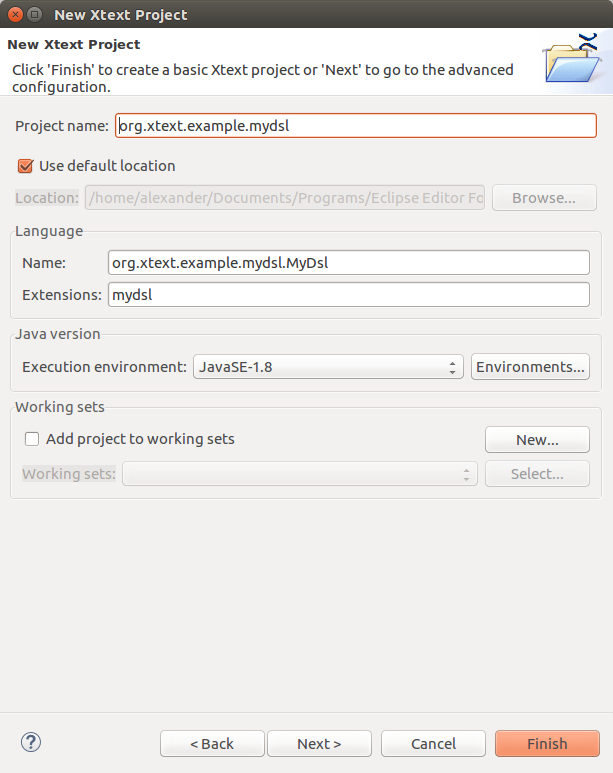
\includegraphics[width=\linewidth]{./Screenshots/newXtextProject.png}
    \caption{page 1}
  \end{subfigure}
  \begin{subfigure}[b]{0.45\linewidth}
    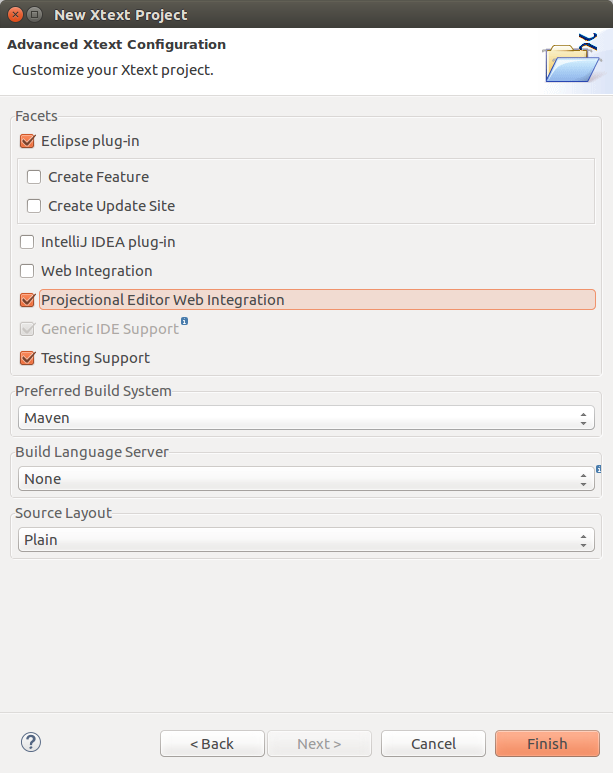
\includegraphics[width=\linewidth]{./Screenshots/newXtextProjectPage2.png}
    \caption{page 2}
  \end{subfigure}
  \caption{The modified "new xtext project" wizard}
  \label{fig:newProjectWiz}
\end{figure}
selecting the "Projectional Editor Web Integration" facet which has been added to the wizard next to the existing option for creating a textual web editor.
\\
\\
This creates an Xtext language project, shown in figure
\begin{figure}[h!]
  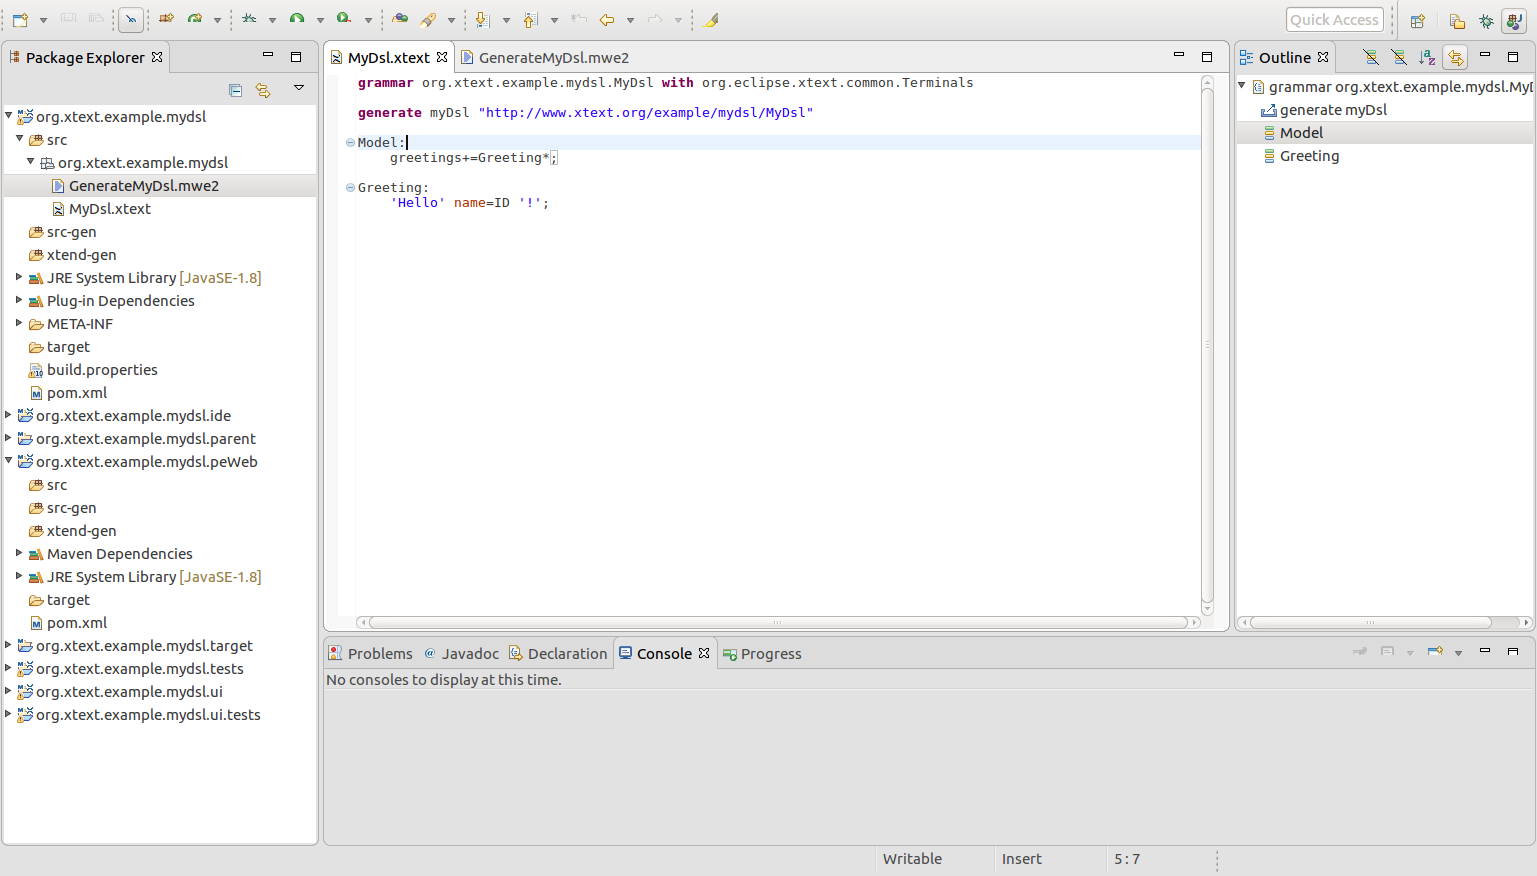
\includegraphics[width=\linewidth]{./Screenshots/newProjectScreen.png}
  \caption{A new xtext project with an empty peWeb project}
  \label{fig:newProjectScreen}
\end{figure} \ref{fig:newProjectScreen}, with a \emph{.xtext} file to specify the DSL's grammar and a \emph{.MWE2} file to describe the generation of the selected facets as usual. A number of empty projects are also created which will contain the files generated by the grammar definition. Notice the \emph{org.xtext.example.mydsl.peWeb} project which has been created and populated with a maven \emph{.pom} file which will be responsible for dependency management and has automatically been configured with the dependencies required by the projectional web editor. 
\\
\\
The generated MWE2 file for the language looks as follows:
\lstinputlisting[ tabsize=2 ]{Listings/GenerateMyDsl.mwe2}
It contains information on the language configuration and how facets for the language should be generated. As we selected the PE facet in the new project notice peWeb is enabled in this file. Because of this, when the user generates the language in the standard Xtext way, by running this MWE2 workflow file, the peWeb project will automatically be populated with all the necessary files to run a server for web based projectional editing. This results in the peWeb project looking like in figure 
\begin{figure}[h!]
  \centering
  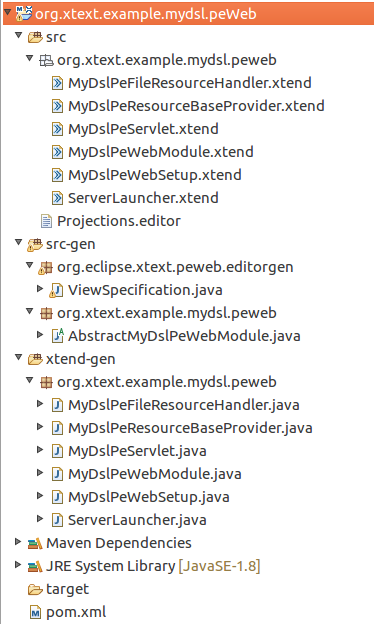
\includegraphics[width=0.4\linewidth]{./Screenshots/peWebProjectContentsAfterGeneration.png}
  \caption{The peweb project following generation}
  \label{fig:generatedPeWebProject}
\end{figure} \ref{fig:generatedPeWebProject}. Notice that MyDsl will be replaced with the name of the created language as specified when creating the project.
These files correspond to the following:
\begin{center}
\begin{tabular}{| m{7cm} | m{8cm} |}
\hline
File & Description \\
\hline \hline
Projections.editor & An empty file in which the language designer can specify the projections for the editor using the \emph{.editor} language discussed later.\\
\hline
MyDslPeServlet.xtend & A HTTP servlet which implements the projectional web API discussed later.\\
\hline
ServerLauncher.xtend & A servlet container to host MyDslPeWebServlet. When ran this starts the language server \\
\hline
MyDslPeFileResourceHandler.xtend & Allows the language designer to specify how files should be read or written, so that any persistence layer can be used. The generated file defaults to simply writing and reading files with the language's extension in the location given by  MyDslResourceBaseProvider \\
\hline
MyDslResourceBaseProvider.xtend & Used to specify how file URI's should be generated for a specified resource in the language. Defaults to a user-files folder at the location of the project.\\
\hline
MyDslPeWebModule.xtend & Allows binding of additional components in the language injector. This is where the resourceHandler and resourceBaseProviders are registered.\\
\hline
MyDslPeWebSetup.xtend & Creates the language injector itself, which will be used to inject information about the specified language into the otherwise generic language server implementation\\
\hline
\end{tabular}
\end{center}
All of the generated files, with the exception of the \emph{Projections.editor} and \emph{MyDslPeServlet}, are required by Xtext's default textual web integration, and so will be familiar to existing XText users. One thing of note is that the FileResourceHandler and ResourceBaseProvider files are not automatically generated in the textual case but are still required. Here by assuming a simple implementation of saving to the local file system, we can generate these files automatically and so enable language designers to get a language server running much more quickly in order to test their language. In fact, at this point, the language designer simply points the serverLauncher to the location of a client application to host (we later present a default such implementation\todo{Reference here}), and the full web editor for their language is ready to run. There is no disadvantage to this generation as these files can be freely changed later or immediately.
%Maybe y generating like this at runtime we can use properties of the language. right now only name but could modify other things too.
%>Fact they are displayed to user means easily extensible matching requirement \RCustom
%>Talk about how the files generated are all commented (TODO) so clear what they are for and so easy to customise \RCustom
%\\
%\\
%\\
%\\
%\\
%\\
%\\
%\\ API
%\\
%\\
%\\
%\\
%\\
%\\
%\\
%\\
%\\
\section{Projectional Editor Web API}\label{api}
In this section I present the design of a server-side web API to allow a client to display and interact with projections for an arbitrary language. It is this API which the generated Projectional Language servers implement in my Xtext extension. It is important to note however that this API is dependent only on the general modelling assumptions I state in \ref{apiAssumptions}, and so is not tied to my Xtext extension and could be implemented by a server generated by any other language workbench or manually created for a general purpose language.

\subsection{Modelling Assumptions}\label{apiAssumptions}
\todo{Better to display this section in terms of a model diagram?}
As this API will be targeting arbitrary languages it is first important to discuss the assumed form of an abstract syntax tree within a programming language. We also must make certain assumptions about the structure of a "project", or collection of files, within that language. As such the following modelling assumptions have been made:
\\
\\
\textbf{Programming Language Definition} = $\{\mathbb{T},\mathbb{D}\}$ 
\begin{itemize}
\item $\mathbb{T}$ - Node Types, a finite set of strings representing the different possible node types which may occur within an AST for the language.
\item $\mathbb{D}$ - Data Types, a finite set of strings representing the different primitive datatypes which may occur within an AST for the language. Note the assumption was made that values of these datatypes are all serialisable as strings, a fair assumption as most languages are entirely driven by the parsing of strings.
\end{itemize}
%
\textbf{Code Project Definition} = $\{n,F \}$ 
\begin{itemize}
\item $n$ - The name of the project as a string
\item $F$ - A set of files (definition below) which this project contains
\end{itemize}
%
\textbf{File Definition} = $\{n, L, a\}$ 
\begin{itemize}
\item $n$ - The name of the file as a string
\item $L=\{\mathbb{T},\mathbb{D}\}$ - The language to be used in this file
\item $a$ - An abstract syntax tree node for the language L which represents the root node of the AST in this file
\end{itemize}
%
Given a language definition $\{\mathbb{T},\mathbb{D}\}$ we define:\\
\\
\textbf{Abstract Syntax Tree Node Definition} = $\{t,C,R,A\}$ 
\begin{itemize}
\item $t\in \mathbb{T}$ - The type of this node in the language
\item $C$ - A finite set of references (definition below), the node's \emph{containment} references, that is the children nodes of this node which may not exist independently of this node. An example in a general purpose language might be a reference to an Expression node from within an If Statement node.
\item $R$ - A finite set of references (definition below), the node's \emph{cross} references, that is references to other nodes which exist independently of this node. An example in a general purpose language may be a Function Call node may cross reference a Function Definition node.
\item $A$ - A finite set of attributes (definition below), the actual data of the node.
\end{itemize}
%
\textbf{Reference Definition} = $\{n,t,R\}$ 
\begin{itemize}
\item $n$ - A string giving the name of this reference.
\item $t\in \mathbb{T}$ - The node type of the nodes being referenced 
\item $R$ - A finite list of AST nodes such that $\{t',C',R',A'\} \in R \implies t'=t$
\end{itemize}
%
\textbf{Attribute Definition} = $\{n,d,A\}$ 
\begin{itemize}
\item $n$ - A string giving the name of this attribute
\item $d\in \mathbb{D}$ - The datatype for the value stored in this attribute
\item $v$ - A value from the datatype $d$
\end{itemize}
%
\subsection{Design}\label{apiDesign}
I now discuss the design of the API itself, giving it's full specification in the appendix \todo{Is it in appendix?}. When designing this API it was necessary to keep in mind the relevant requirements for the project's ultimate goal as given in \ref{requirements}. The goal to produce a lightweight (\RLightweight) and customisable (\RCustom) editor are clearly relevant here and so the API was designed with these in mind.
\\
\\
The first consideration was how best to transport the state of the abstract syntax tree between client and server. Existing solutions in textual web editing, such as within LSP or Xtext's own default web editor implementation rely on first synchronising the client with the server by sending the full contents of a document opened as a string. Further requests or edits are then handled by referencing positions within the document as line/position numbers or ranges. This pattern of synchronisation followed by incremental updates between client and server has the advantage of minimising the amount of data required to be transmitted. In order to do this on ASTs directly however we need some way of referencing nodes within a tree. We achieve this by annotating each node within an AST on the server side with a unique identifier. If the client is then aware of this labelling we can use it to communicate incremental changes between client and server, such as changes to attribute values.
\\
\\
Having decided upon this annotation of the ASTs in order to reference incremental updates, we next look at the initial synchronization. In order to keep the client application as lightweight as possible (as per \RLightweight) we wish to minimise the data synchronised onto the client. We notice that the client only ever needs to maintain state relating to the parts of the AST(s) that they are actively interacting with. With a textual representation, this is very difficult to determine, and by default we assume the user wishes to display the entire textual contents of a file. However, a projectional editor has no such issue. At any given time a user is interacting only with projections of the AST, these projections define explicitly which nodes of the AST, and which attributes within these, are relevant and should be displayed. Hence we have no need to synchronise all details of the AST with the client initially, only as and when these are required by a projection.
\\
\\
With this in mind then, initial synchronisation happens as follows. Upon opening a file the client application requests a "skeleton" tree, consisting only of node names (generated by the language server, perhaps using certain attribute values or the node's type) and their unique identifiers. This can be used for navigation within the file, enabling the user to request projections for subtrees they wish to edit instead of for the whole file. Through some means then, a subtree is selected to be displayed, the client makes a request to fetch that subtree's root node using the id from the client's skeleton tree, and the server responds with the attributes and references which will be displayed within the projection for that node in some format. From here we are ready to begin transmitting only incremental changes made within this projection between client and server. In the case that the user wishes to edit a different subtree we can then ask for the values relevant to that node using it's id from the skeleton tree which we can keep cached.
\todo{Include a diagram here}
\\
\\
\subsubsection{Transferring Node State}
To actually display and interact with an AST on the client side it needs both information about the current state of the relevant nodes, and how to project this state so that the user can interact with it. 
There are two approaches to doing this which place different requirements on the client side application. The first is to require that the client application itself has definitions for the possible projection types, and so given the state of a node and the name of the projection to use it can create the projection itself. The other option is for information about the projection to be sent along with the state of the node, so the client application need not know anything about the language or projections it may use at compile time as these are supplied by the language server.
\\
\\
Both approaches have advantages, the first allows for more flexibility in the projections that can be written, and if a projection is to be used by many nodes reduces the amount of data to be retrieved from the language server. The second approach however keeps the size of the client application much smaller, especially if the language is large and requires many different projection types. Since projection specification is inherently associated with a language, it is also the case that only the second approach allows a client application to remain language independent while still being able to display language specific projections.
\\
\\
Because both have advantages, in line with our \RCustom requirement to allow as much flexibility as possible for language designers, we decide to design this API such that both approaches are possible.
\\
\\
To achieve this the API specifies that a node fetch response should simply be as an arbitrary Json object with a type field. The client should be capable of decoding the object based upon it's type. We then specify two language independent node-fetch types in this project which can be assumed to be standard, and should prove sufficient for most use cases. Language designers can still however create new node-fetch types for the language server to use, provided they extend the client application accordingly to handle these new types.
\\
\\
The two standard types are:
\begin{itemize}
\item \emph{Default Projection}: The client is given all the attributes and references for the node which it then presents to the user in any meaningful way as decided by the client application.
\item \emph{CustomHtml Projection}: This method involves sending not only relevant attributes for the node to the client, but also sending html to specify how it should be projected. The intention is that these will be automatically generated by the projection specification language given in section \ref{EditorLanguage}, as such they will be discussed in more detail there.
\end{itemize}

\subsubsection{Making Changes to a Node}

We notice from our modelling assumptions that a node consists of a series of attributes, \textit{containment} reference features and \textit{cross-reference} reference features. In order to make changes to nodes we thus provide 3 methods in our API to modify these things. Each method takes as parameter the project name, file name and nodeId of the node being modified so that the server doesn't have to store state regarding which nodes clients have requested and are editing. The methods are as follows: 
\begin{itemize}
\item \emph{update-attribute} : Takes the attribute name  of the node and it's new value (as a string, using our assumption here that all datatypes in a language are serialization as such). 
\item \emph{add-reference} : Takes the reference feature name as a parameter. In the case of a cross-reference we also expect a child-id parameter, that is, the node identifier of the node we wish to cross reference, the language server then adds this reference. In the case of a containment reference no additional parameters are required and the language server creates a new node of the type specified by the reference feature's type. The language server assigns this a fresh identifier and sends the skeleton subtree rooted at this new node back to the client so it may update it's skeleton tree. (This response allows the language server to create children for the newly created node if required as a side-effect)
\item \emph{remove-reference} : Takes the reference feature name and id of the node to remove as parameter. It then removes the reference from the feature, and if it was a part of a containment reference then it deletes the node from the tree and removes all cross references to it from other nodes.
\end{itemize} 
%\\
%\\
Following the update of a node we can check that we have left it in a valid state using the \emph{validate-node} method which takes as parameter the project name, file name and nodeId of a node and returns an object which either signals that the node is in a valid state OR that it isn't and a string with the error message. In the case of removing a containment reference, as other nodes may have cross referenced it, we must instead use the \emph{validate} method, which will return a list of every node which is not in a valid state with the matching error strings.

\subsection{Implementation in Xtext}
I now talk about how this API is implemented in the language servers that are automatically generated for DSL specifications in my Xtext extension.
\\
\\
The generated server hosts a Java HTTP servlet. In order to make API calls the client is expected to send get requests to the url pattern specified by the language designer in the generated \emph{MyDslPeServlet.xtend} file, which, by default, is /pe-service/. The client uses a http parameter serviceType to choose the API call to make, and adds other parameters to the request as required by the API call made. The server responds with standard http error codes if there is a mistake with the request parameters or in the execution of the method or otherwise with a json object containing the response of the call.
\\
\\
In order to get files and project details, the language server injects the FileResourceHandler and ResourceBaseProvider objects specified in the \emph{MyDslPeFileResourceHandler.xtend} and \emph{MyDslResourceBaseProvider.xtend} files. These objects define operations to get and save EMF resources from a "resource id" (we use PROJECTNAME/FILENAME) so that arbitrary persistence layers can be used. By default these correspond to storing files in their textual representation at /user-files/PROJECT_NAME/FILE_NAME.LANGUAGE_EXTENSION relative to the language server, so that loading a file is equivalent to parsing the stored textual representation into an AST and saving uses the parser rules to create a textual representation from the AST. Retrieving a file using the method in the FileResourceHandler results in an EMF Resource object, from which we can retrieve the EObject which represents the root node of the AST that file represents.
\\
\\
The EObject retrieved closely matches an AST as we described in our modelling assumptions, containing reference features linking to other EObjects and attributes. When we first open a file and retrieve it's EObject all that remains then is to annotate the tree with unique identifiers as discussed in \ref{apiDesign} which we do recursively from the root. We also construct two additional maps, one from these identifiers to the respective annotated node, and another from the EObjects themselves to the nodeIds. The first of these maps allows us to efficiently find nodes referenced by API calls, the second allows us to find the nodeId of a node even if we obtain it by following the unannotated EObject's references directly. These maps are kept up to date incrementally as nodes are added and removed from the tree.
\\
\\
Modifying nodes is then done by looking up the relevant node using the nodeID to EObject map and then making the relevant changes to the EObject itself.
%EObject contains all the attributes and reference types as well as some constraints on the node so already have AST in effect
%From these nodes we create a tree where children of a node are all those contained only in containment references, that is every node is only in this tree once
%We annotate it with node identifiers which we do when we first open the file
%We also create a map from these  nodeIds to the EObjects themselves
%We also create a map in the other direction, so if we follow a reference in the EObject we can easily look up the node id if we need to communicate this with the client
%This is all cached and kept up to date incrementally as the tree changes
%Modifying nodes is all done by looking up the nodes with the nodeId-> eobject map and then modifying the eobject directly
%\\
%\\
%\\
%\\
%\\
%Insert Editor Language
%\\
%\\
%\\
% Views
\todo{This section}







\printbibliography

\end{document}
